4\chapter{Iteración 4: “Reportes de incidentes y acciones automáticas”}
    En Security Onion y otros sistemas, el elemento descriptor que identifica y procesa a cada definición de incidente en particular es la regla. Las reglas comprenden una serie de campos que describen con precisión la naturaleza de un incidente dado y por lo tanto, existen tantas reglas como amenazas en circulación. \par
    Cuando un nuevo malware es descubierto por el equipo de algún CSIRT con la capacidad de investigación suficiente o reportado a un laboratorio apropiado para este fin, es posible realizar un estudio de sus características y una vez identificadas estas últimas, proceder a crear una regla y agregarla al repositorio correspondiente para que otros CSIRT actualicen sus IDS con esta nueva definición y así contar con un filtro (la regla) que permita detectar este malware. Las reglas tienen un conjunto de campos donde se detallan características del paquete y su contexto, tales como el puerto de origen y destino, protocolo empleado, dirección IP, etc y unos campos dedicados a la naturaleza del incidente (clasificación, mensaje, prioridad, etc). Algunos de estos campos son comunes a todas las reglas y permiten agruparlas para administrar eficientemente las alertas generadas cuando una regla coincide con la descripción de un incidente. Dado que estos campos también se pueden considerar observables, es posible utilizarlos por TheHive y Cortex para automatizar respuestas. \par

    \begin{section}{Análisis de prioridades de los incidentes}
    Como se indicó anteriormente, la estructura de las reglas consisten en dos partes bien definidas: un encabezado (header) que es obligatorio  y un conjunto de campos opcionales. Dentro del header encontramos la acción (alerta, notificación, etc), el protocolo (tcp, udp), puertos de origen y destino, el sentido del evento (entrante o bidireccional) y las direcciones IP de origen y destino. \par
    La segunda parte de las reglas incluye dos tipos de campos: los que describen la naturaleza del evento y aquellos que contienen información del paquete de datos. Dentro del primer grupo encontramos aquellos tales como msg (descripción del evento), sid (id de la firma), classtype (clasificación de reglas o alertas), priority (prioridad de la firma y/o alerta), target (especifica de qué lado está el objetivo, es decir puerto de origen y puerto de destino), entre otros. El segundo grupo contiene datos extraídos que provienen desde de la capa de red hasta la de aplicación de la pila OSI. Se pueden mencionar a los campos “GeoIP” (localización geográfica de la IP), “Fragbits” (presencia del bit de fragmentación), “ACK” (presencia del campo ACK en paquete TCP), “itype” (número del tipo de mensaje ICMP), “http.method” (tipo de método HTTP usado), entre otros.
     \begin{figure}[H]
        \centering
        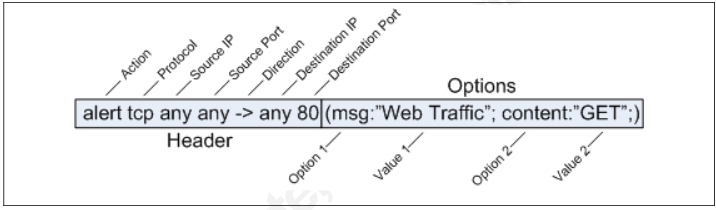
\includegraphics[width=0.7\textwidth]{./iteracion_3_imagenes/figura_41_estructura_regla.png}
        \caption{Estructura general de una regla}
        \label{fig:figura_41_estruc_regla}
     \end{figure}
    
    Como se describió en los párrafos precedentes, como los campos están presentes en todas las reglas, es posible hacer uso de algunos de ellos para agrupar reglas que describen amenazas pertenecientes a un mismo grupo o categoría de malware, intentos de intrusión, reconocimiento, escalado de privilegios, etc y por lo tanto son útiles para gestionar los incidentes. \par
	Es posible configurar esta gestión a través de un archivo que relaciona campos como categorías de eventos con prioridades de la alerta generada. Este archivo llamado “classification.config” se encuentra bajo el directorio que almacena las reglas descargadas desde diversas fuentes; en particular relaciona los campos “classtype” con “priority”, de manera tal que cualquier regla cuyo campo classtype contenga a los descritos en este archivo, generará una alerta con prioridad definida también en este. De esta manera, es posible administrar un enorme número de reglas agrupadas en un reducido grupo de categorías y modificar el nivel de prioridad que tendrá en el sistema las alertas que generan. \par
	El objetivo de asignar distintos niveles de prioridad a las alertas generadas por los eventos que sucedan radica en la naturaleza de los eventos, su importancia y la gestión de la atención de los analistas del CSIRT. Esto se debe a las necesidades de optimizar el uso de los recursos técnicos y humanos del centro de respuesta a incidentes para cumplir de la manera más eficiente posible con los objetivos y políticas de la organización a la cual pertenece. De esta manera, la naturaleza de los incidentes determina su elegibilidad para una respuesta automatizada al tener en cuenta por un lado su estructura bien conocida y por el otro su alta tasa de repetición en un periodo determinado. En estos casos, sería inutil destinar valiosos recursos como la atención de un analista ya que conoce perfectamente la estructura del incidente y por lo tanto la respuesta apropiada o en aquellos casos en los que aún conocida su estructura, el incidente proviene en simultáneo de múltiples fuentes en muy poco tiempo, de manera que la capacidad humana de responder de a uno a la vez estaría tan sobrepasada que no sería efectiva. Estos son los casos de ataques de reconocimiento y los de denegación distribuida de servicio, entre otros. \par
	De aproximadamente cuarenta y siete (47) categorías de incidentes disponibles por defecto, consideramos para el máximo nivel de prioridad a siete clasificaciones dado su nivel de ocurrencia y nivel de impacto para la organización. 
    \begin{itemize}
        \item Web-application-attack: esta categoría engloba a un conjunto enorme de malware y ataques a nivel de capa de aplicación. Gusanos, ransomware, ataques de reconocimiento entre otras amenazas comparten esta categoría. Sobre el caso particular de los ataques de reconocimiento, se aplicaron filtros para separarlos de los demás ya mencionados. 
        \item Unsuccessful User: intentos repetidos de ganar acceso en ciertos activos e infraestructura de la organización.
        \item Attempted-dos: intentos de ataque de denegación de servicio y su variante distribuida
        \item Known client side exploit attempt: intento de ejecución de exploits en el lado del cliente.
        \item Exploit Kit Activity Detected: detección de actividad de un kit de exploits
        \item A suspicious filename was detected: detección de nombres de archivos sospechosos
        \item Network Trojan: detección de un virus troyano de red.
    \end{itemize}
    \end{section}